\subsection{Перемена порядка интегрирования. Сведение кратных интегралов к повторным (Теоремы Тонелли и Фубини)}
Далее мы считаем, что зафиксированы два пространства с $\sigma$-конечными полными мерами $(X, \MM, \mu)$ и $(Y, \NN, \nu)$ и их тензорное произведение $(X \times Y, \ \MM \otimes \NN, \ \mu \otimes \nu)$.
\begin{corollary}[Геометрический смысл интеграла Лебега б/д]
    Пусть $f: X \rightarrow \overline{\R}$~---~измеримая функция. Тогда определим $\Gamma_f = \{(x, t) \in X \times \R \mid t = f(x) \}$ и для неотрицательных $f$ определим подграфик: $$\Pi_f = \{(x, t) \in X \times \R \mid 0 \leq t \leq f(x) \}.$$ Из принципа Кавальери следует следующее:
    \begin{itemize}
        \item $\mu \otimes \LL^1(\Gamma_f) = 0$.
        \item Для неотрицательной функции измеримость в широком смысле эквивалентна измеримости её подграфика. Более того, $\mu \otimes \LL^1(\Pi_f) = \int\limits_X fd\mu$.
    \end{itemize}

\begin{minipage}{0.5\textwidth}\raggedleft
Интеграл Лебега это буквально площадь под графиком неотрицательной измеримой в широком смысле функции(те где-то может быть неопределена)
\end{minipage}    
\begin{minipage}{0.5\textwidth}% adapt widths of minipages to your needs
    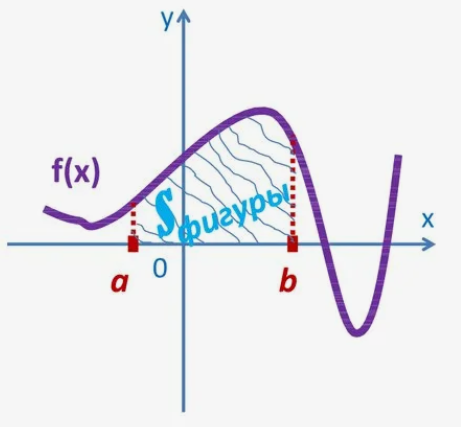
\includegraphics[width=0.5\textwidth]{images/Integral.png} 
\end{minipage}%

\end{corollary}
\hfill%

\begin{definition}
    Пусть $f$: $X \times Y \rightarrow \overline{\R}$. Зафиксируем одну из переменных и оставим вторую переменную. Это буквально значение функции на сечении. Определим следующие функции: 

\begin{minipage}{0.5\textwidth}\raggedleft
    \[\forall x \in X:\quad f_x (\cdot): Y \rightarrow \overline{\R}, \  y \mapsto f(x, y);\]
    \[\forall y \in Y: \quad f^y(\cdot): X \rightarrow \overline{\R}, \ x \mapsto f(x, y).\]
\end{minipage}
    \begin{minipage}{0.5\textwidth}% adapt widths of minipages to your needs
    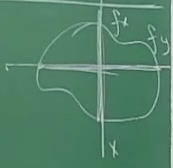
\includegraphics[width=0.4\textwidth]{images/Slice.png}
\end{minipage}%
\hfill%
 

\end{definition}
\begin{theorem}[Тонелли]
    Пусть $f$~---~неотрицательная $\MM\otimes\NN$-измеримая функция на $X \times Y$. Тогда верны следующие утверждения:\\
    (!) Важно, что функция неотрицательная.
    \begin{enumerate}
        \item[1а)] Для $\mu$-п.в. $x \in X \hookrightarrow f_x$~---~измерима на $Y$;
        \item[1б)] Для $\nu$-п.в. $y \in Y \hookrightarrow f^y$~---~измерима на $X$.
        \item[2а)] $\phi: x \mapsto \int\limits_Y f_xd\nu$~---~измеримая в широком смысле функция на $X$;
        \item[2б)] $\psi: y \mapsto \int\limits_X f^yd\mu$~---~измеримая в широком смысле функция на $Y$.
        \item[3)] Справедливо равенство: \[\int\limits_{X \times Y}f(x, y)d(\mu\otimes\nu)(x, y) = \int\limits_X\biggl(\int\limits_Y f_x (y) d\nu (y) \biggr)d\mu(x) = \int\limits_Y\biggl(\int\limits_X f^y(x)d\mu(x)\biggr)d\nu(y).\]
    \end{enumerate}
\end{theorem}
\begin{proof}
Идея доказательства. Любая измеримая функция является пределом простых. Докажем для характеристической функции измеримого множества с использованием принципа Кавальери. Произвольная простая функция является линейной комбинацией харфункций. Далее с помощью теоремы Леви перейдем к пределу. \\
\underline{Шаг 1.} Пусть $f = \chi_C,$ где $ C \in \MM \otimes \NN$. Значит, фиксируя $\forall x \in X $, получим $ f_x = \chi_{C_x}$, поскольку 
\[f_x(y) = f(x, y) = \chi_C(x, y) = \begin{cases}
    1, & (x, y) \in C \\ 0, & (x, y) \notin C
\end{cases} = \begin{cases}
    1, & y \in C_x \\ 0, & y \notin C_x
\end{cases} = \chi_{C_x}(y).\]
Но $x$ выбран произвольно, тогда из п.1 принципа Кавальери следует что при $\mu$-п.в. $x \in X \hookrightarrow f_x$~---~измерима. Так как наша функция это характеристическая функция множества, то её интеграл~---~мера множества. Тогда из п.2 принципа Кавальери следует измеримость в широком смысле функции $\phi$, а из п.3 \[ \mu \otimes \nu (C) = \int\limits_{X \times Y} X_C(x, y)d(\mu\otimes\nu)(x, y) = \int\limits_X \nu(C_x)d\mu(x) = \int\limits_X\biggl(\int\limits_Y f_xd\nu\biggr)d\mu.\] что и требовалось доказать. \\
\underline{Шаг 2.} Если $f$~---~произвольная простая неотрицательная функция, то по определению $\exists \{a_1, \ldots, a_n\} \subset [0, +\infty)$ и $E_1, \ldots E_n \subset X. \  (E_i \cap E_j = \emptyset, i\neq j)$ такие, что $f = \sum\limits_{k = 1}^n a_k\chi_{E_k}$ выполнение всех пунктов теоремы следует из предыдущего шага и линейности интеграла Лебега для неотрицательных функций. \\
\underline{Шаг 3.} В общем случае, для неотрицательной измеримой функции $f$ существует неубывающая последовательность простых функций $\{f_n\}_{n=1}^{\infty}$, т.ч. $f_n \rightarrow f, n \rightarrow +\infty$.\\
Для любого $n \in \N$, для $\mu$-п.в. $x \in X$ функция $(f_n)_x$~---~$X \times Y$-измерима. Для каждого $n$ множество где, $(f_n)_x$ не определено свое, но их счётное объединение является множеством нулевой меры. Тогда и $\mu$-п.в. $x \in X \ \forall n \in \N \hookrightarrow  (f_n)_x$~---~измерима. Тогда $(f)_x$ измерима как поточечный предел измеримых и монотонно растущих. Тогда по теореме Леви мы получаем: \[\phi(x) = \int\limits_Y f_x(y)d\nu(y) = \lim\limits_{n \rightarrow +\infty} \int\limits_Y (f_n)_x(y) d\nu(y).\]
Тогда, поскольку $\forall n \in \N \   \phi_n: x \mapsto \int\limits_Y (f_n)_xd\nu$ измерима в широком смысле, то и её предел $x \mapsto \int\limits_Y f_xd\nu$ тоже измерим в широком смысле как предел при $\mu$-п. в. $х \in X$. Из монотонности $\{f_n\}$ и монотонности интеграла по функциям мы получаем монотонность последовательности $\{\phi_n\}$. Таким образом, можно ещё раз воспользоваться теоремой Леви и получить следующее: \[\int\limits_X \phi d\mu = \lim\limits_{n \rightarrow +\infty} \int\limits_X \phi_n d\mu = \lim\limits_{n \rightarrow +\infty} \int\limits_X \biggl(\int\limits_Y (f_n)_xd\nu\biggr)d\mu = \lim\limits_{n \rightarrow +\infty} \int\limits_{X \times Y} f_n d\mu\otimes\nu = \int\limits_{X \times Y} fd(\mu\otimes\nu) .\]
Что и требовалось доказать. Для $f^y$ доказательство аналогично.\\
\end{proof}
\begin{note}
    Как следует рассматривать теорему Тонелли? Часто довольно сложно посчитать двойной интеграл. Мы переставили пределы как нам нужно, получили конечное. Тогда теорема Тонелли говорит что и при других перестановках будет конечное значение и это все будет равно интегралу. Т.е. обе части либо меньше бесконечности, либо равны бесконечности одновременно
\end{note}

\begin{theorem}[Фубини]
    Пусть $f$~---~интегрируемая на $X \times Y$ по $\mu \otimes \nu$ функция $f \in \widetilde{L_1}(X \times Y, \mu \otimes \nu)$. То есть $\int\limits_{X\times Y} f d(\mu \otimes \nu) < +\infty$. Тогда справедливо следующее:
    \begin{enumerate}
        \item[1а)] Для $\mu$-п.в. $x \in X \hookrightarrow f_x$~---~интегрируема на $Y$;
        \item[1б)] Для $\nu$-п.в. $y \in Y \hookrightarrow f^y$~---~интегрируема на $X$.
        \item[2а)] $\phi: x \mapsto \int\limits_Y f_xd\nu$~---~интегрируема по $\mu$;
        \item[2б)] $\psi: y \mapsto \int\limits_X f^yd\mu$~---~интегрируема по $\nu$.
        \item[3)] Верно следующее равенство: \[\int\limits_{X \times Y}fd\mu\otimes\nu = \int\limits_X \phi d\mu = \int\limits_Y \psi d\nu.\]
    \end{enumerate}
\end{theorem}
\begin{proof}
    Пусть $f = f_+ - f_-$. Воспользуемся теоремой Тонелли для $f_+$ и $f_-$: \[\int\limits_{X \times Y}f_\pm d(\mu\otimes\nu) = \int\limits_X\biggl(\int\limits_Y (f_\pm)_xd\nu \biggr)d\mu < +\infty.\]
    По ней же $(f_\pm)_x$~---~измеримы, а $(\phi_\pm)_x$~---~измеримы в широком смысле, где $\phi_\pm = \int\limits_Y f_\pm(x, y) d\nu(y)$. Т.к. $\int\limits_X \phi_\pm d\mu < +\infty$, то $\phi_\pm$~---~интегрируемы, а значит п.в. конечны, а значит $(f_\pm)_x$~---~интегрируемы при п.в. $x \in X$. Третий пункт теоремы следует из линейности интеграла Лебега.
\end{proof}
\begin{note}
    Разница между теоремами:
    \begin{itemize}
        \item     Теорема Тонелли утверждает, что для неотрицательных функций можно менять порядок интегрирования и гарантирует равенство интегралов. Вне зависимости от конечности интеграла
        \item Теорема Фубини расширяет это утверждение на случай функций, которые могут принимать как положительные, так и отрицательные значения, при условии конечности интеграла.
    \end{itemize}
\end{note}
\begin{note}
    Может быть так, что существуют повторные интегралы (более того -- они могут быть равны), но при этом $f$~---~не интегрируема по $\mu \otimes \nu$.
\end{note}
\begin{example}
    Пусть \[f(x, y) = \begin{cases}
        \dfrac{x^2 - y^2}{(x^2 + y^2)^2}, & x^2 + y^2 > 0 \\
        0, & x^2 + y^2 = 0 
    \end{cases}\]
    $f$ не интегрируема на $[-1, 1]^2$ по $\LL^1 \otimes \LL^1$, но существуют повторные интегралы.
\end{example}
\begin{example}
    Пусть \[f = \begin{cases}
        \dfrac{xy}{(x^2 + y^2)^2}, & x^2 + y^2 \neq 0 \\
        0, & x^2 + y^2 = 0
    \end{cases}\]
    Эта функция не интегрируема по $\LL^1 \otimes \LL^1$, но, при этом,  существуют повторные интегралы, равные $0$.
\end{example}
\subsection{Мера Лебега как произведение мер}
\begin{theorem}
    Пусть $m, n \in \N$. Тогда $\LL^n \otimes \LL^m = \LL^m \otimes \LL^n = \LL^{m + n}$ и $\MM^n \otimes \MM^m = \MM^m \otimes \MM^n = \MM^{m + n}$.
\end{theorem}
\begin{proof}
    По определению, $\LL^{m + n}$~---~стандартное продолжение по Каратеодори меры $\lambda_{m + n}$, определённой на $\PP^{m + n}$~---~полукольце стандартных ячеек в $\R^{m + n}$. \\
    По определению произведения мер, $\LL^n \otimes \LL^m$~---~стандартное продолжение меры $$m(E \times G) = \LL^n(E)\cdot\LL^m(G)$$ на полукольце $\PP$ множеств вида $E \times G, E \in \MM^n, G \in \MM^m,$ где $ \LL^n(E) < +\infty, \LL^m(G) < +\infty$. Тут нужно почувствовать разницу, ведь в первом случае берутся  $n+m$ мерные ячейки, а во втором различные декартовы произведения конечных множеств конечной меры, которые тоже образуют полукольцо. Понятно что это разные полукольца, но не сильно :) \\
    Пусть $m^*$~---~внешняя мера, порождённая $m$, $\lambda_{m + n}^*$~---~внешняя мера, порождённая $\lambda_{m + n}$. \\
    По ранее доказанной теореме, $m^* \leq \lambda_{m + n}^*$ (т.к. $\PP^{m + n} \subset \PP$). \\
    Пусть $E$~---~множество конечной меры $m^*$. Тогда существует $\{P_j\} \subset \PP$ т.ч. \[\sum\limits_{j = 1}^\infty m(P_j) \leq m^*(E) + \epsilon\]
    Тогда $\forall P_j = E_j \times G_j$ каждый из них измерим в своей сигма алгебре:
    \[
    \sum\limits_{j = 1}^\infty m(P_j) =  \sum\limits_{j = 1}^\infty \LL^n(E_j) \LL^m(G_j).
    \]
    В силу регулярности меры Лебега $\LL^n$ и $\LL^m$, $\exists U_i, W_i$~---~открытое $:U_i\supset E_i$ и $W_i \supset G_i$ т.ч. \[\sum\limits_{i = 1}^\infty \LL^n(U_i)\LL^m(W_i) < m^*(E) + \epsilon.\]
\begin{fact}
    Любое открытое в $\R^n$ реализуется в виде не более чем счетного дизъюнктивного объединения ячеек с рациональными центрами и рёбрами.
\end{fact}
    Пусть $\{P_i\}_{i = 1}^\infty$~---~ячейки в $\R^n$, $\{Q_j\}_{j = 1}^\infty$~---~ячейки в $\R^m$. По определению меры ячейки $\LL^n(P_i)\LL^m(Q_i) = \LL^{m + n}(P_i \times Q_i)$. Тогда $\LL^{n + m}(U_i \times W_i) = \LL^n(U_i)\LL^m(W_i)$, т.к. $U_j \times W_j$~---~открытое множество. $E \subset \bigcup_{j=1}^{\infty} P_i \times Q_j \subset \bigcup_{j=1}^{\infty} U_j \times W_j$   \\
    Таким образом мы получаем \[\lambda^*_{n+m}(E) \leq \sum\limits_{i = 1}^\infty \lambda^*_{n+m} (U_j \times W_j) = \sum\limits_{i = 1}^\infty \LL^{n+m} (U_j \times W_j) = \sum\limits_{i = 1}^\infty \LL^{n} (U_j) \LL^{m}(W_j) <  m^*(E) +\epsilon\]
    В силу произвольности $\epsilon > 0$  получаем необходимое неравенство для произвольного множества конечной внешней меры: \[\lambda^*(E) < m^*(E)\]
    Тогда $\lambda^* = m^*$ и теорема доказана.
\end{proof}

% Быть может, параграф <<мера Лебега как произведение мер стоит поправить>>

\section{Замена переменной в интеграле Лебега}
\subsection{Изменение меры Лебега при отображениях}
\begin{reminder}
    Отображение $F: E \rightarrow \R^m$, где $E \subset \R^n$ называется липшицевым, если $\exists L > 0$, т.ч. $\forall x, y \hookrightarrow \|F(x) - F(y)\| \leq L\|x - y\|$. Пишем, что $F \in \LIP(E, \R^m)$. Наименьшая такая $L$ называется константой Липшица и обозначается как $L_F$.
\end{reminder}
\begin{fact}
    Пусть $F \in \mathcal{C}^1(\mathcal{O}, \R^m), \mathcal{O}$~---~открытое в $\R^n$. Тогда $F$ локально липшецево, т.е. для любого выпуклого компакта $K$ в $\mathcal{O} \   \exists L(K) > 0$ т.ч. $F \in \LIP(K, \R^m), L_F = L(K)$.
\end{fact}
\begin{theorem}
    Пусть $\mathcal{O}$ это открытое в $\R^n$ множество. Пусть $F \in \mathcal{C}^1(\mathcal{O}, \R^n)$. Пусть $E \subset \mathcal{O}$~---~$\LL^n$-измеримо. Тогда $F(E)$~---~измеримо по Лебегу.
\end{theorem}
\begin{proof}
    В силу регулярности меры Лебега \[E = \bigcup\limits_{j = 1}^\infty K_n \cup e,\]
    где $K_n$~---~возрастающая последовательность компактов, а $e$~---~множество меры нуль. Из непрерывности $F$ следует, что $F(K_n)$~---~компакт. Тогда \[F\biggr(\bigcup\limits_{j = 1}^\infty K_n \cup e\biggr) = \bigcup\limits_{j = 1}^\infty F(K_n) \cup F(e).\]
    Поскольку счётное объединение компактов~---~борелевское множество, для измеримости образа достаточно показать, что $F(e)$~---~измеримо. Покажем, что $\LL^n(F(e)) = 0$. Предположим, что существует ячейка $P \in \PP^n$: $e \subset \overline{P} \subset \mathcal{O}$. Тогда из липшицовости $F$ на $\overline{P}$ существует константа Липшица $L$. В то же время, поскольку $\LL^n(e) = 0$, то $\forall \epsilon > 0$ существует последовательность ячеек $\{Q_j\}$: $\sum\limits_{n = 1}^\infty \LL^n(Q_j) < \epsilon$.
%я на 45 странице, через 5 часов проснусь и продолжу
%тут бы ещё центры указать
\begin{fact}
    Любая ячейка представляется в виде дизъюнктного объединения кубических ячеек c рациональными ребрами и рациональным центром.
\end{fact}
    Тогда $\exists \  \{\Pi_l\}$ т.ч. \[e \subset \bigsqcup\limits_{l = 1}^\infty \Pi_l, \ \sum\limits_{l = 1}^\infty \LL^n(\Pi_l) = \sum\limits_{l = 1}^\infty (h_l)^n < \epsilon.\]
    Т.к. $diam(F(\Pi_l)) \leq Ldiam(\Pi_l) \leq Lh_l\sqrt{n}$,
    то $F(\Pi_l) \subset B_{Lh_l\sqrt{n}} \subset \Pi_{2Lh_l\sqrt{n}} = T_l$. Тогда \[\lambda^*(F(e)) \leq \sum\limits_{l = 1}^\infty \LL^n(T_l) \leq \sum\limits_{l = 1}^\infty (2Lh_l\sqrt{n})^n \leq C\cdot\sum\limits_{l = 1}^\infty \LL^n(\Pi_l) \leq C\epsilon\]
    В силу произвольности $\epsilon > 0$ мы получаем, что $\lambda^*(F(e)) = 0$, тк мера Лебега полна, то $F(e)$ измеримо те $\LL^n(F(e)) = 0$. Если же $e$ не содержится внутри одной ячейки, то мы можем разбить $\mathcal{O}$ на счётное объединение ячеек, и повторить данное рассуждение для пересечения $e$ с каждой из ячеек. Поскольку счётное объединение множеств меры нуль имеет меру нуль, мы получаем необходимое. 
\end{proof}
\subsection{Трансляционная инвариантность меры Лебега}
\begin{theorem}
    Пусть $E$~---~измеримое по Лебегу в $\R^n$. Тогда $\forall v \in \R^n$ верно следующее: $v + E$~---~измеримо и $\LL^n(v + E) = \LL^n(E)$.
\end{theorem}
\begin{proof}
    Пусть $v \in \R^n$. Рассмотрим отображение $F: x \mapsto x + v$. Так как оно гладко, то $v + E = F(E)$~---~измеримо. Для доказательства неизменности меры рассмотрим новую меру $\mu(E) = \LL^n(E + v)$.  $\forall E \in \MM_n = \bigsqcup_{k=1}^{\infty}E_k$
    \[
    \mu(E) = \LL^n( v + \bigsqcup_{k=1}^{\infty} E_k) = \sum_{k=1}^{\infty}\LL^n(v + E_k) = \sum_{k=1}^{\infty}\mu(E_k)
    \]
    Эти меры очевидно совпадают на полукольце ячеек. А значит меры это продолжение, по единственности продолжения совпадают на пересечении $\sigma$-алгебр, то есть просто совпадают.
\end{proof}

\begin{theorem} Любая трансляционно инвариантная мера в $\R^n$ совпадает с мерой Лебега с точностью до константы. Пусть $\mu$~---~трансляционно инвариантная мера, определённая на $\MM^n$ и конечная на компактах. Тогда \[\forall E \in \MM^n \hookrightarrow \mu(E) = \mu \big([0, 1)^n \big)\cdot\LL^n(E) =  k \cdot \LL^n(E) \]
\end{theorem}
\begin{proof}
    Если мера $\mu([0, 1)^n) = 0$, то в силу трансляционной инвариантности мы получаем, что $\mu \equiv 0$. \\
    Если мера $\mu([0, 1)^n) = 1$, то для того, чтобы доказать $\mu \equiv \LL^n$ на $\MM^n$ достаточно это проверить на кубических ячейках рационального радиуса. Любую кубическую ячейку можно получить как сдвиги и в силу трансляционной инвариантности достаточно доказать 
$$\mu([0, 1/k)^n) = 1/k^n\mu \big([0, 1)^n \big) = 1/k^n$$что в точности совпадает с мерой кубической ячейки. \\
    Если мера $\mu([0, 1)^n) = k \neq 1$, то пусть $\nu = \mu/k$. Тогда $\nu([0, 1)^n) = 1$, а значит $\nu \equiv \LL^n$ и $\mu = k\LL^n$.
\end{proof}